\subsection{Graph Theory}

In graph theory, a \textit{graph} is defined as containing both a set of \textit{vertices} and a set of \textit{edges} disjoint from each other, with the restriction that the set of vertices is non-empty, as well as an \textit{incidence function} which associates an unordered pair of vertices with each edge \citep{Bondy1976}. A graph $G$ can be represented as
\begin{align*}
    G = (V(G), E(G), \psi_{G}),
\end{align*}
where $V(G)$ is the set of vertices, $E(G)$ is the set of edges, and $\psi_{G}$ is the incidence function \citep{Bondy1976}. A \textit{bipartite graph} is a specific type of graph wherein the vertex set can be partitioned into two subsets $X$ and $Y$ such that every edge in the edge set has one end in $X$ and the other in $Y$ \citep{Bondy1976}, i.e. no vertices in the same set $X$ or $Y$ can be connected by an edge. Examples are shown in Figure \ref{fig:graphs}.

%\afterpage{
    \begin{figure}[t]
    \centering
    \begin{subfigure}{.5\textwidth}
        \centering
        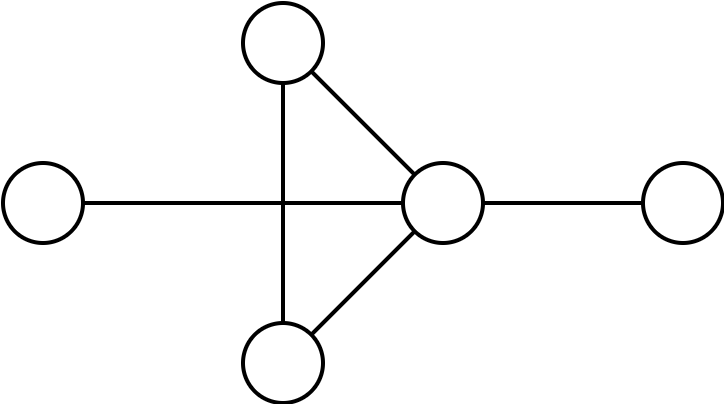
\includegraphics[height = .15\textheight]{basicgraph}
        \caption{A simple, non-bipartite graph.}
        \label{fig:simplegraph}
    \end{subfigure}%
    \begin{subfigure}{.5\textwidth}
        \centering
        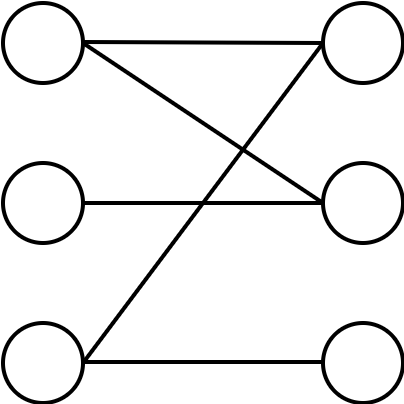
\includegraphics[height = .15\textheight]{bipartitegraph}
        \caption{A simple, bipartite graph.}
        \label{fig:bipartitegraph}
    \end{subfigure}
    \caption{Two examples of a graph structure where vertices are connected by edges. The circles represent vertices and the lines between circles represent edges. Note that the bipartite graph can be represented by a partition of the vertices into two subsets such that there are no edges between vertices in the same subset.}
    \label{fig:graphs}
    \end{figure}
%}

\begin{figure}[t]
    \centering
    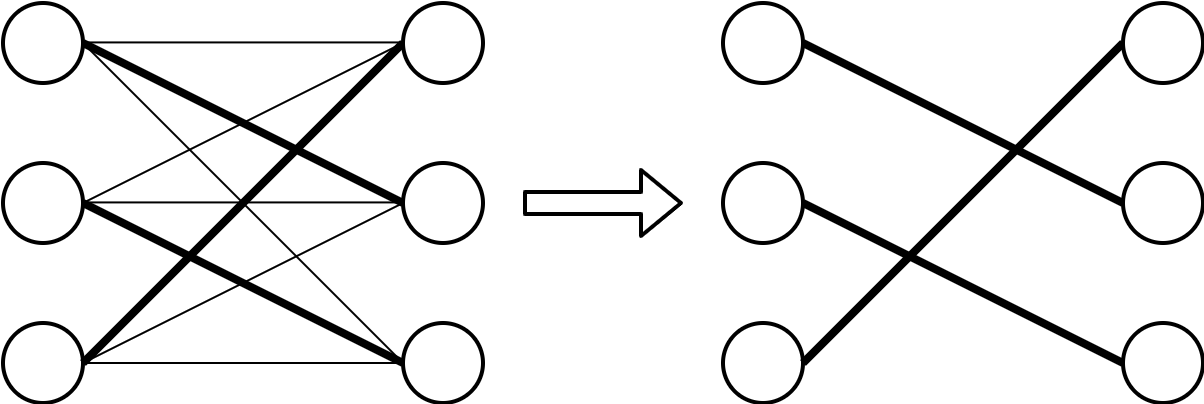
\includegraphics[height = .1575\textheight]{perfectmatching.png}
    \caption{An example of a perfect matching in a 3-regular bipartite graph where no member of the matching is incident with the same vertex as another member and all vertices in the graph are incident with at least one member of the matching. Members of the perfect matching are represented by bold lines.}
    \label{fig:perfectmatching}
\end{figure}

A graph is considered $k$-regular if each vertex in the graph is adjacent to exactly $k$ other vertices. This can also be referred to as each vertex having a \textit{degree} of $k$ and denoted as $d_{G}(v) = k$ for all $v \in V(G)$. A \textit{perfect matching} is a set of edges in a graph such that each vertex in the graph is incident to an edge from the perfect matching, but no two edges in the perfect matching are incident with the same vertex. This concept is demonstrated in Figure \ref{fig:perfectmatching}. If a graph is both $k$-regular and bipartite for some $k > 0$, it must contain a perfect matching \citep{Bondy1976}.

Consider a graph where each vertex represents a person and the edges between two vertices represent an expression of interest between two people. Note that an expression of interest is not a pairing. Additionally, let this graph be both $k$-regular and bipartite for some $k > 0$. Then there must exist a perfect matching within this graph. This allows us to pair each member of one partition with a member of the other partition in a manner analogous to a stable marriage \citep{Bondy1976}. Thus, we can consider finding a perfect matching within a $k$-regular, bipartite graph to be a solution to the stable marriage problem in the instance where each expressed interest is equally weighted.

Whereas set theory is inadequate for applying the stable marriage to Tinder, graph theory is sufficient for doing so. Let $T$ be a bipartite graph representative of Tinder. Let the set $X$ be the entirety of Tinder's user base such that each vertex represents a single user and let the set $Y$ be a copy of the same user base. Then let $T$ be a bipartite graph with the vertex set $X \cup Y$. Note that each user is then represented by two vertices in $T$. Let the edges between vertices represent a reciprocal expression of interest between users, i.e a \textit{match} as it is referred to by Tinder. For now, we will assume that a user has equal preference between all matches. If $T$ could be shown to be $k$-regular (also referred to as just \textit{regular}), then it could be stated that a stable marriage exists inside of Tinder. However, it may not be necessary for $T$ to be regular in order to guarantee the existence of a stable marriage.

\begin{figure}[t]
    \centering
    
\includegraphics[height = .30\textheight]{h1andh2.png}
    \caption{A bipartite graph $T$ decomposed into two subgraphs $H_{1}$ and $H_{2}$ such that each subgraph is regular and $H_{1}$ and $H_{2}$ are both disjoint and edge-disjoint from each other. The degree of a vertex, where a vertex represents a user and an edge between vertices represents an expression of interest, is represented by the number adjacent to the vertex.}
    \label{fig:h1andh2}
\end{figure}

A graph $H$ is defined as a subgraph of a graph $G$ if $V(H) \subseteq V(G)$, $E(H) \subseteq E(G)$, and $\psi_{H}$ is the restriction of $\psi_{G}$ to $E(H)$ \citep{Bondy1976}. Additionally, we can consider two subgraphs $H_{1}$ and $H_{2}$ to be disjoint if they share no vertices and edge-disjoint if there are no edges that connect the vertices from $H_{1}$ to the vertices of $H_{2}$ and vice versa \citep{Bondy1976}. If it can be shown that $T$ can be decomposed into the two subgraphs $H_{1}$ and $H_{2}$ and that both $H_{1}$ and $H_{2}$ satisfy the stable marriage problem, then it would be shown that $T$ still satisfies the stable marriage problem even if $T$ itself is not regular. An example of this decomposition can be seen in Figure \ref{fig:h1andh2}. Note however that $T$ does not necessarily have to be decomposed into only two subgraphs. This notion is extended into the following theorem.

\begin{theorem}
\label{theorem:smsg}
Let $G$ be composed of bipartite subgraphs that are both disjoint and edge-disjoint such that for sets $X$ and $Y$ of any subgraph the members of $X$ have ranked only the members of $Y$ in order of preference and vice versa. Assume a lack of preference is equivalent to the worst possible preference. Then the assignment of members in $G$ is a stable marriage if the assignment of members in each subgraph is a stable marriage.
\end{theorem}
\begin{proof}
Let $H_{\alpha}$ and $H_{\beta}$ be two distinct subgraphs of $G$ such that all members of a subgraph have been paired with another member of the same subgraph. Then, without loss of generality, for any $\alpha \in H_{\alpha}$ there is no element in $H_{\beta}$ that $\alpha$ will prefer to its current assignment. This implies that there exists no $g_{1}, g_{2} \in G$ such that both $g_{1}$ and $g_{2}$ would rather be assigned to each other than their current partner. Thus, the assignment of members in $G$ is a stable marriage.
\end{proof}

It is difficult, if not impossible, to determine if Tinder satisfies the conditions for Theorem \ref{theorem:smsg}. However, we argue that if enough regular subgraphs of sufficient size exist within Tinder's representative graph $T$, then consequently enough stable marriages may exist to greatly diminish Tinder's user base. After all, the formation of regular subgraphs is not unlikely. Tinder tailors a user's experience to their own personal preferences, such that the user will generally not encounter people who fall outside these preferences \citep{Courtois2018}. This greatly limits the recommendation pool for the user and, thus, it is likely that users with similar preferences will cluster together into smaller subgraphs or \textit{communities}. If these users all match with each other the community would then become regular when observed independently of the larger graph.

We note that there is no guarantee that these communities are disjoint or edge-disjoint from each other. Indeed, considering that a person can belong to multiple communities, the small world effect \citep{Newman2003} would seem to argue that any two communities are connected by a chain of an average length of six people. This is a seemingly non-existent distance compared to the millions of people that use Tinder. However, a lack of distinction may not be enough to completely throw out Theorem \ref{theorem:smsg}. For example, if all members of a community prefer each other over members of another community and vice versa, the two communities are equivalently disjoint, as the members' top interests are contained within a single community, and edge-disjoint, as removing the edges between these two subgraphs would have no effect on a stable marriage algorithm. Thus, a high count of regular communities in $T$ could pose a potential problem for Tinder. This gives us the following corollary.

\begin{corollary}
\label{corollary:subgraphs}
A graph which can be partitioned into regular subgraphs that are disjoint but not necessarily edge-disjoint may still satisfy Theorem \ref{theorem:smsg} if the edges between two subgraphs represent a preference weaker than all preferences in both subgraphs.
\end{corollary}

This corollary will be relied on heavily in later sections. However, one large issue remains with this model. It was assumed that users will have equal preference for each other, but this is a generous assumption that does not follow reality. While graph theory does possess the tools to overcome this assumption, concepts from network science will provide a more complete model.